
\documentclass[a4 paper,12pt]{article}
\usepackage[inner=2.0cm,outer=2.0cm,top=2.5cm,bottom=2.5cm]{geometry}
\usepackage{setspace}
\usepackage{appendix}
\usepackage[rgb]{xcolor}
\usepackage{tabu}
\usepackage{multirow}
\usepackage{longtable}
\usepackage{graphicx}
\usepackage{verbatim}
\usepackage{longtable}
\usepackage{subcaption}
\usepackage{fancyhdr}
\usepackage[colorlinks=true, urlcolor=blue, linkcolor=blue, citecolor=blue]{hyperref}
\usepackage{booktabs}
\usepackage{amsmath,amsfonts,amsthm,amssymb}
\usepackage{setspace}
\usepackage{fancyhdr}
\usepackage{lastpage}
\usepackage{tikz}
\usepackage{listings}
%\lstset{
	%	commentstyle=\color{red!50!green!50!blue!50},%代码块背景色为浅灰色
	%	rulesepcolor= \color{gray}, %代码块边框颜色
	%	breaklines=true,  %代码过长则换行
	%	numbers=left, %行号在左侧显示
	%	numberstyle= \small,%行号字体
	%	keywordstyle= \color{blue},%关键字颜色
	%	frame=shadowbox,%用方框框住代码块
	%	basicstyle=\ttfamily
	%}
\definecolor{dkgreen}{rgb}{0,0.6,0}
\definecolor{mauve}{rgb}{0.9,0.1,0.4}
\definecolor{ash}{rgb}{0.8,0.8,0.8}
\lstset{ 
	language=Octave,                % the language of the code
	basicstyle=\ttfamily,           % the size of the fonts that are used for the code
	numbers=left,                   % where to put the line-numbers
	numberstyle=\small\color{gray},  % the style that is used for the line-numbers
	stepnumber=2,                   % the step between two line-numbers. If it's 1, each line
	% will be numbered
	numbersep=5pt,                  % how far the line-numbers are from the code
	backgroundcolor=\color{ash},      % choose the background color. You must add \usepackage{color}
	rulesepcolor= \color{gray}, %代码块边框颜色
	showspaces=false,               % show spaces adding particular underscores
	showstringspaces=false,         % underline spaces within strings
	showtabs=false,                 % show tabs within strings adding particular underscores
	frame=single,                   % adds a frame around the code
	rulecolor=\color{black},        % if not set, the frame-color may be changed on line-breaks within not-black text (e.g. commens (green here))
	tabsize=2,                      % sets default tabsize to 2 spaces
	captionpos=b,                   % sets the caption-position to bottom
	breaklines=true,                % sets automatic line breaking
	breakatwhitespace=false,        % sets if automatic breaks should only happen at whitespace
	title=\lstname,                   % show the filename of files included with \lstinputlisting;
	% also try caption instead of title
	frame=shadowbox,%用方框框住代码块
	keywordstyle=\color{blue},          % keyword style
	commentstyle=\color{dkgreen},       % comment style
	stringstyle=\color{mauve},         % string literal style
	escapeinside={\%*}{*)},            % if you want to add LaTeX within your code
	morekeywords={*,...}               % if you want to add more keywords to the set
}
\usetikzlibrary{positioning, arrows.meta}
\usepackage{extramarks}
\usepackage{ctex,amsmath,amsfonts,amssymb,bm,hyperref,graphicx}
\usepackage{chngpage}
\usepackage{soul,color}
\usepackage{graphicx,float,wrapfig}
\newcommand{\homework}[3]{
	\pagestyle{myheadings}
	\thispagestyle{plain}
	\newpage
	\setcounter{page}{1}
	\noindent
	\begin{center}
		\framebox{
			\vbox{\vspace{2mm}
				\hbox to 6.28in { {\bf 现代电子电路基础及实验报告 \hfill} {\hfill {\rm #2} {\rm #3}} }
				\vspace{4mm}
				\hbox to 6.28in { {\Large \hfill #1  \hfill} }
				\vspace{3mm}}
		}
	\end{center}
	\vspace*{4mm}
}
\newcommand\numberthis{\addtocounter{equation}{1}\tag{\theequation}}

\begin{document}
	\homework{TTL与非门参数测量}{1900011413}{吴熙楠}
	
	\section{实验目的}
	(1)了解 TTL 与非门参数的意义和使用注意事项;
	\par (2) 学习 TTL 非门参数的测量方法。
	\section{实验器材}
	直流稳压电源、示波器、信号发生器、万用表、面包板 、电阻、电位器、TTL芯片。
	\section{实验原理}
    \noindent
\textbf{3.1电压传输特性及干扰能力}
\par 与非门的输出电压$V_{o}$随输入电压$V_{i}$的变化关系,称为电压传输特性如图所示:
	\begin{figure}[H]
		\centering
		\hspace{2em}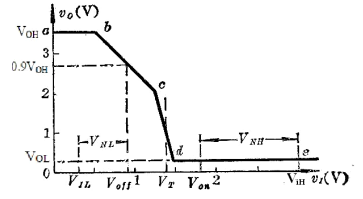
\includegraphics[width=.6\linewidth]{pic/1.png}
		\caption{电压传输特性曲线
		}
	\end{figure}
\par 其中,$V_{iL}$为输入低电压,$V_{iH}$为输入高电压,$V_{oL}$为输出低电压,$V_{oH}$为输出高电压,$V_{off}$为关门电压,$V_{on}$为开门电压,$V_{T}$为门限电压,$V_{NL}$为低电平容限,$V_{NH}$为高电平容限。电平传输特性描述了与非门的静态特性,$V_{off}$ 和 $V_{on}$的差值愈小,则表明与非门的电压传输特性愈陡直,静态开关性能愈好,其抗干扰能力愈强。\\
\noindent
\textbf{3.2空载功耗}
\par 空载功耗是与非门不接外部负载时,电源电流 $I_{o}$ 与电源电压 $E_{c}$ 的乘积,它是估算电路内耗的参量。通常只测定静态功耗,即在输入端全开路时的功耗 $P_{on}$和短路时的功耗$P_{off}$,前者为空载导通功率,后者为空载截止功率,测试电路如下图所示:
	\begin{figure}[H]
		\centering
		\hspace{2em}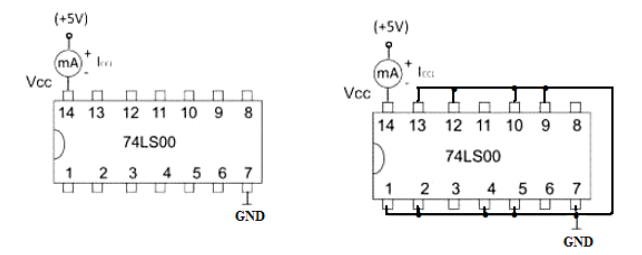
\includegraphics[width=.6\linewidth]{pic/2.png}
		\caption{$P_{on},P_{off}$的测试电路
		}
	\end{figure}
\noindent
\textbf{3.3输入短路电流}
\par $I_{is}$ 是指与非门的一个输入端接地,其余输入端接高电平或开路时,流向接地端的电流,$I_{is}$称为输入短路电流,测试电路如下图所示:
	\begin{figure}[H]
		\centering
		\hspace{2em}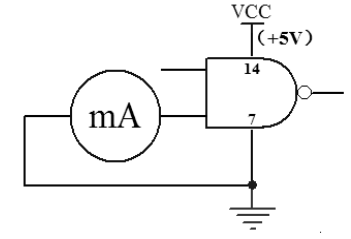
\includegraphics[width=.35\linewidth]{pic/3.png}
		\caption{$I_{is}$的测试电路
		}
	\end{figure}
\noindent
\textbf{3.4输入交叉漏电流}
\par $I_{iH}$是指与非门的一个输入端接高电平,其余输入端接地时,流入高电平输入端的电流,测试电路如下图所示:
	\begin{figure}[H]
		\centering
		\hspace{2em}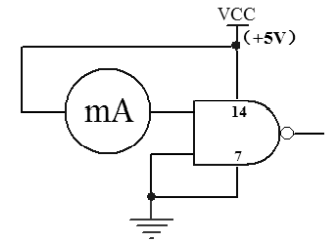
\includegraphics[width=.35\linewidth]{pic/4.png}
		\caption{$I_{iH}$的测试电路
		}
	\end{figure}
\noindent
\textbf{3.5输出低电平 $V_{oL}$和输出高电平 $V_{oH}$}
\par $V_{oL}$是指当输入为高电平,输出端接额定灌电流负载时(相当于八个与非门的 $I_{is}$),与
非门的输出电压值。$V_{oH}$是指当输入为低电平、输出端接额定拉电流负载时(相当于八个与非门的$I_{iH}$),与非门的输出电压值。\\
\noindent
\textbf{3.6扇出系数$N_{c}$}
\par 扇出系数 $N_{c}$定义为前级门低电平最大输出电流(灌电流)和后级门低电平最大输入电流的比值。$N_{c}$ 是说明与非门输出端负载能力的参数,它表示能驱动同类门的数目,测试电路如下图所示:
	\begin{figure}[H]
		\centering
		\hspace{2em}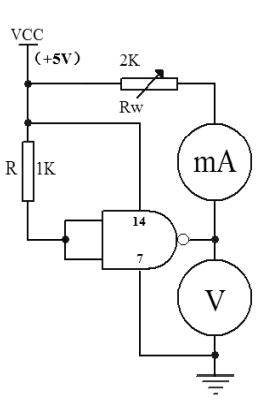
\includegraphics[width=.3\linewidth]{pic/5.png}
		\caption{$V_{oL}$和$N_{c}$的测试电路
		}
	\end{figure}
\noindent
\textbf{3.7平均传输延迟时间$t_{pd}$}
\par 传输延迟时间是指与非门的输出信号的延时,$t_{pd}$ 是门电路的重要参量,由于存在延迟时间,一方面可能产生"冒险"等有害的伪信号,另一方面也可利用延时的效应,组成某些电路(如环形振荡器)。
	\section{实验内容}
    \noindent
    \textbf{4.1验证与非门的逻辑功能}
    \par 各门输入端悬浮,测得各输出端的电压为:$U_{1}=0.1700V,U_{2}=0.1670V,U_{3}=0.1528V,U_{4}=0.1672V$,与非门输出全为低电平。
    \par 各门输入端接地,测得各输出端的电压为:$U_{1}=4.4857V,U_{2}=4.4897V,U_{3}=4.4917V,U_{4}=4.4872V$,与非门输出全为高电平。\\
    \noindent
    \textbf{4.2空载功耗$P_{ON}$和$P_{OFF}$}
    \par 测量电路如图2,我们可以测得$I_{ON}=2.1768mA,I_{OFF}=0.2124mA,U=5V$
    \par 所以$P_{ON}=UI_{ON}=10.884mW,P_{OFF}=UI_{OFF}=1.062mW$\\
    \noindent
    \textbf{4.3输入短路电流$I_{is}$}
    \par 测量电路如图3,我们可以测得$I_{is}=0.2340mA$\\
    \noindent
    \textbf{4.4交叉漏电流$I_{iH}$}
    \par 测量电路如图4,由于测量精度的原因,我们未能测得交叉漏电流$I_{iH}$,即$I_{iH}\le 10^{-4}mA$.
    \clearpage
    \noindent
    \textbf{4.5扇出系数$N_{c}$}
    \par 测量电路如图5,我们可以测得$I_{L}=7.2683mA$,因此我们可得$N_{c}=\dfrac{I_{L}}{I_{is}}\approx 31.06$\\
    \noindent
    \textbf{4.6三级环形振荡器}
    	\begin{figure}[H]
    		\centering
    		\hspace{2em}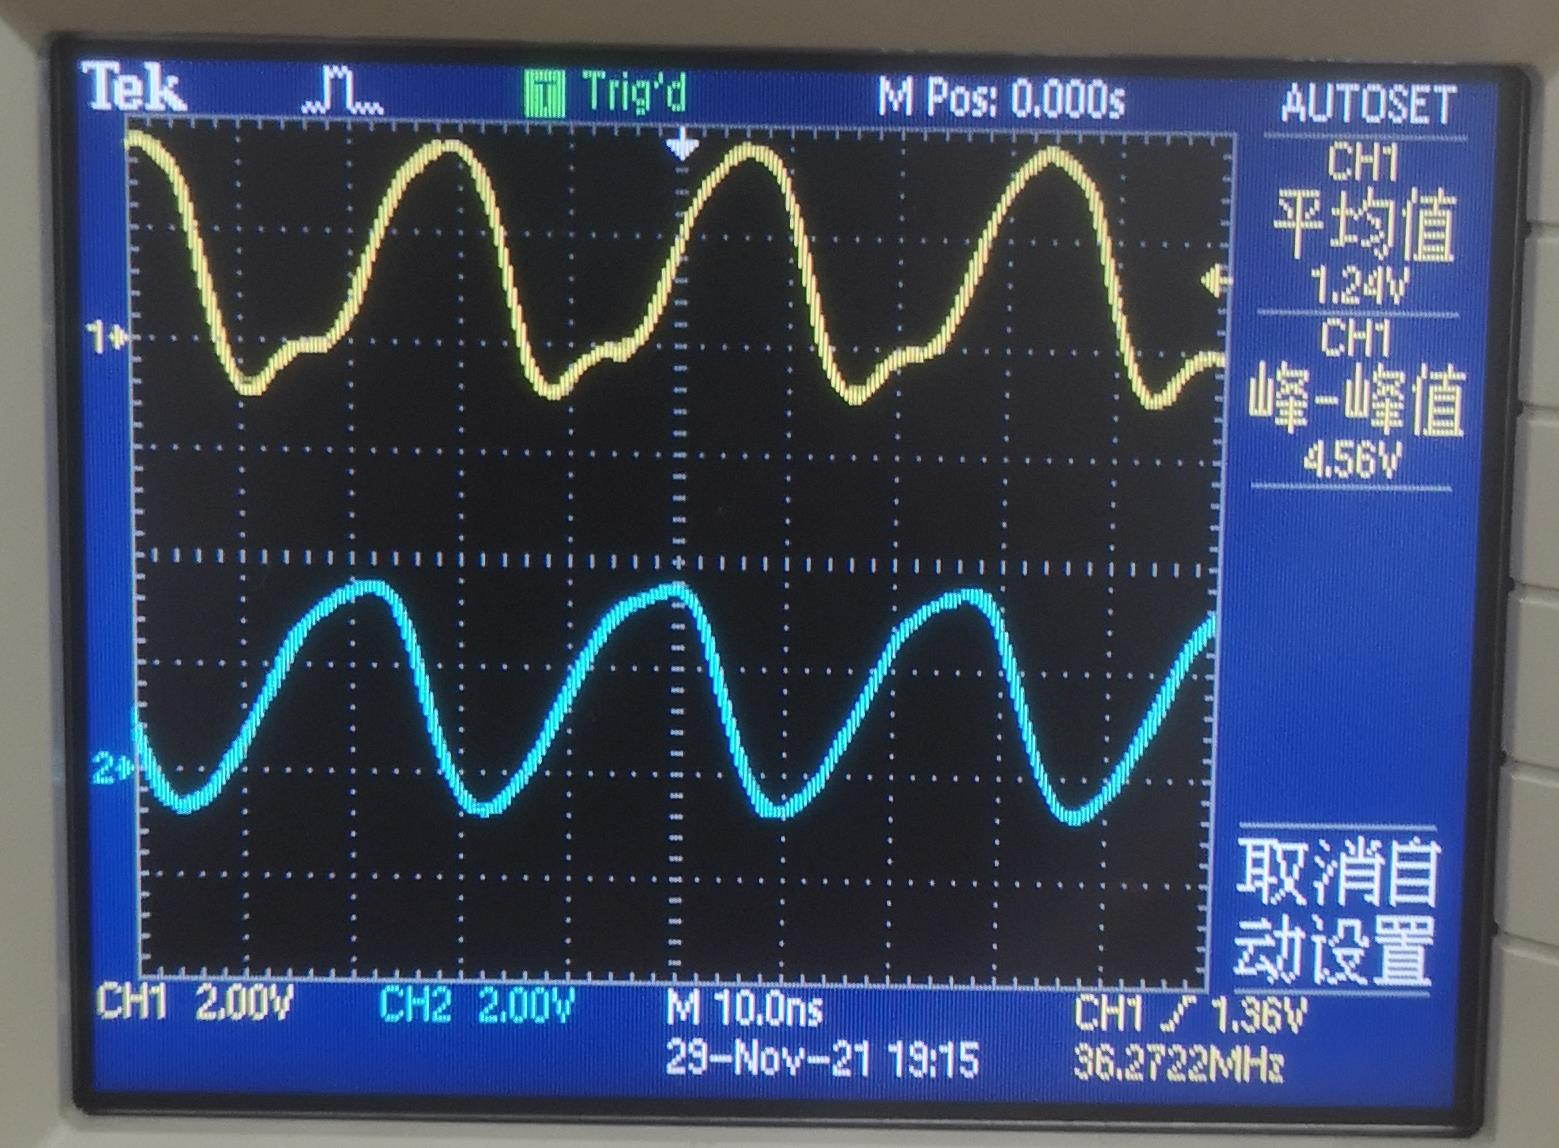
\includegraphics[width=.4\linewidth]{pic/1.jpg}
    		\caption{三级环形振荡器波形图
    		}
    	\end{figure}
        \par 由图中我们可以得到振荡频率$f\approx 36.2722MHz$\\
    \noindent
    \textbf{4.7利用计数器电路分频}
    	\begin{figure}[H]
    		\centering
    		\hspace{2em}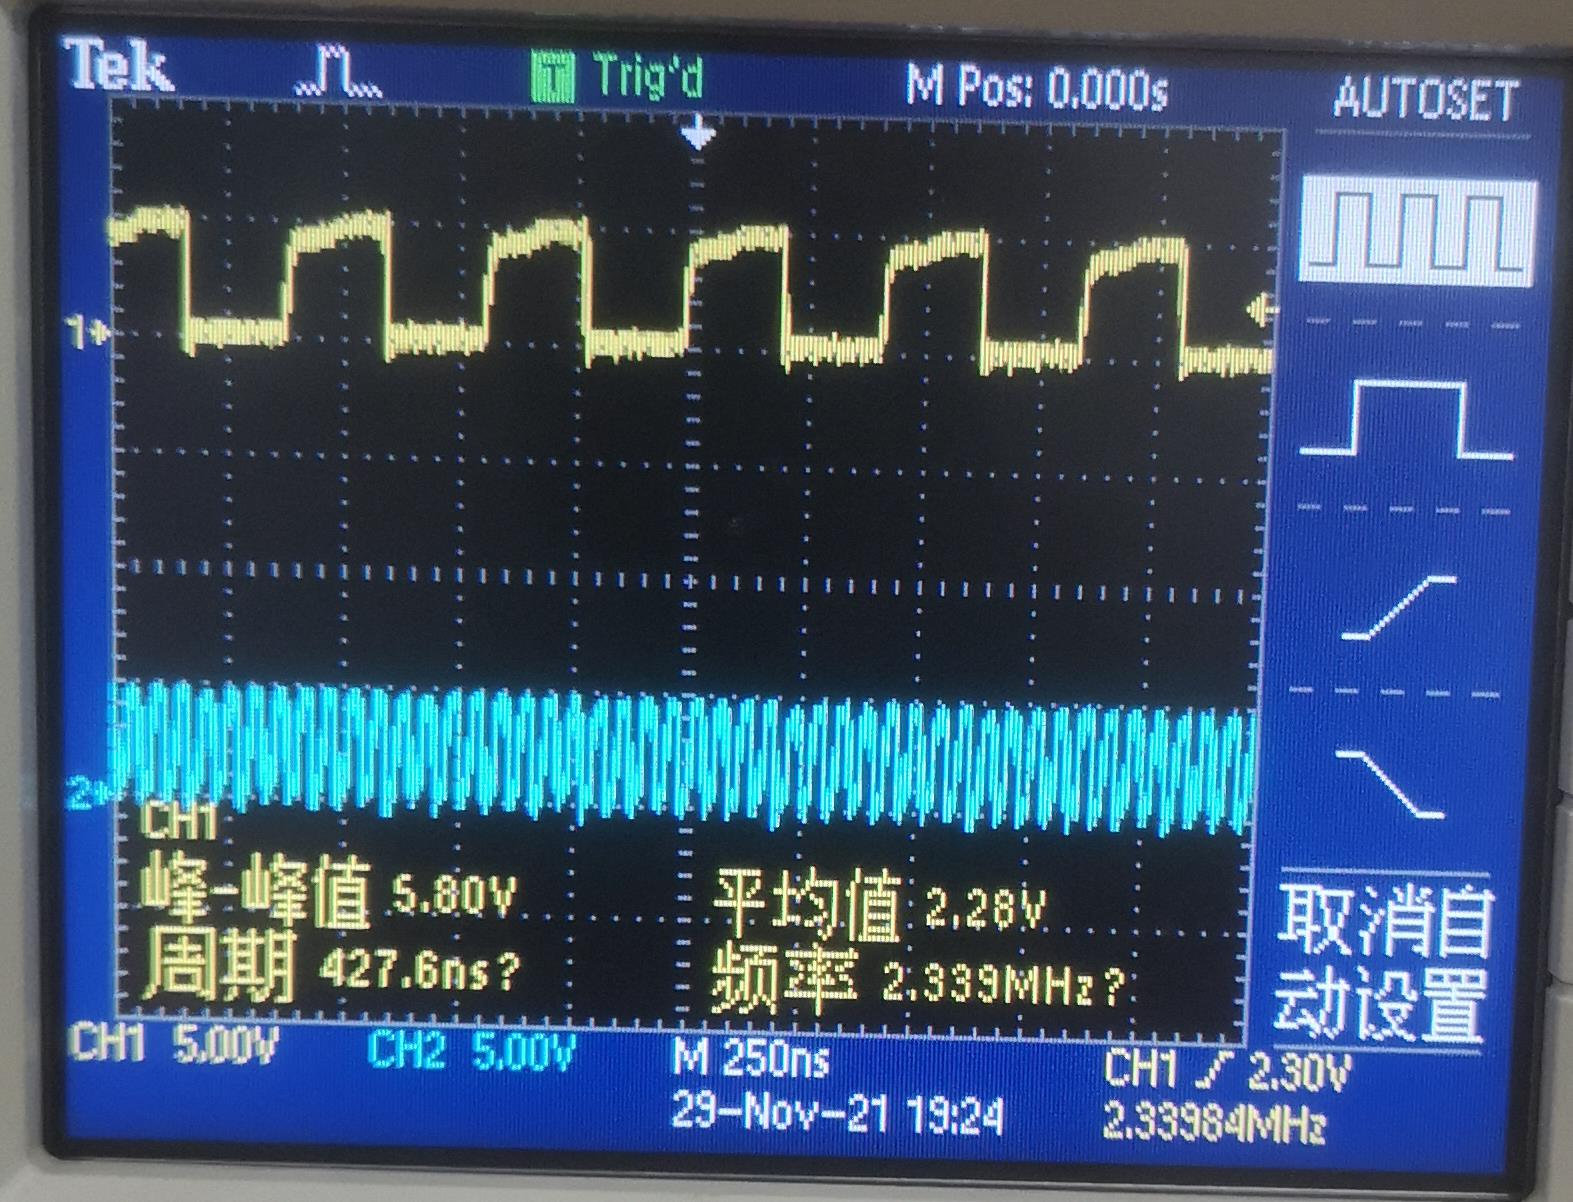
\includegraphics[width=.4\linewidth]{pic/2.jpg}
    		\caption{$Q_{A}$和$Q_{D}$波形图
    		}
    	\end{figure}
    	\begin{figure}[H]
    		\centering
    		\hspace{2em}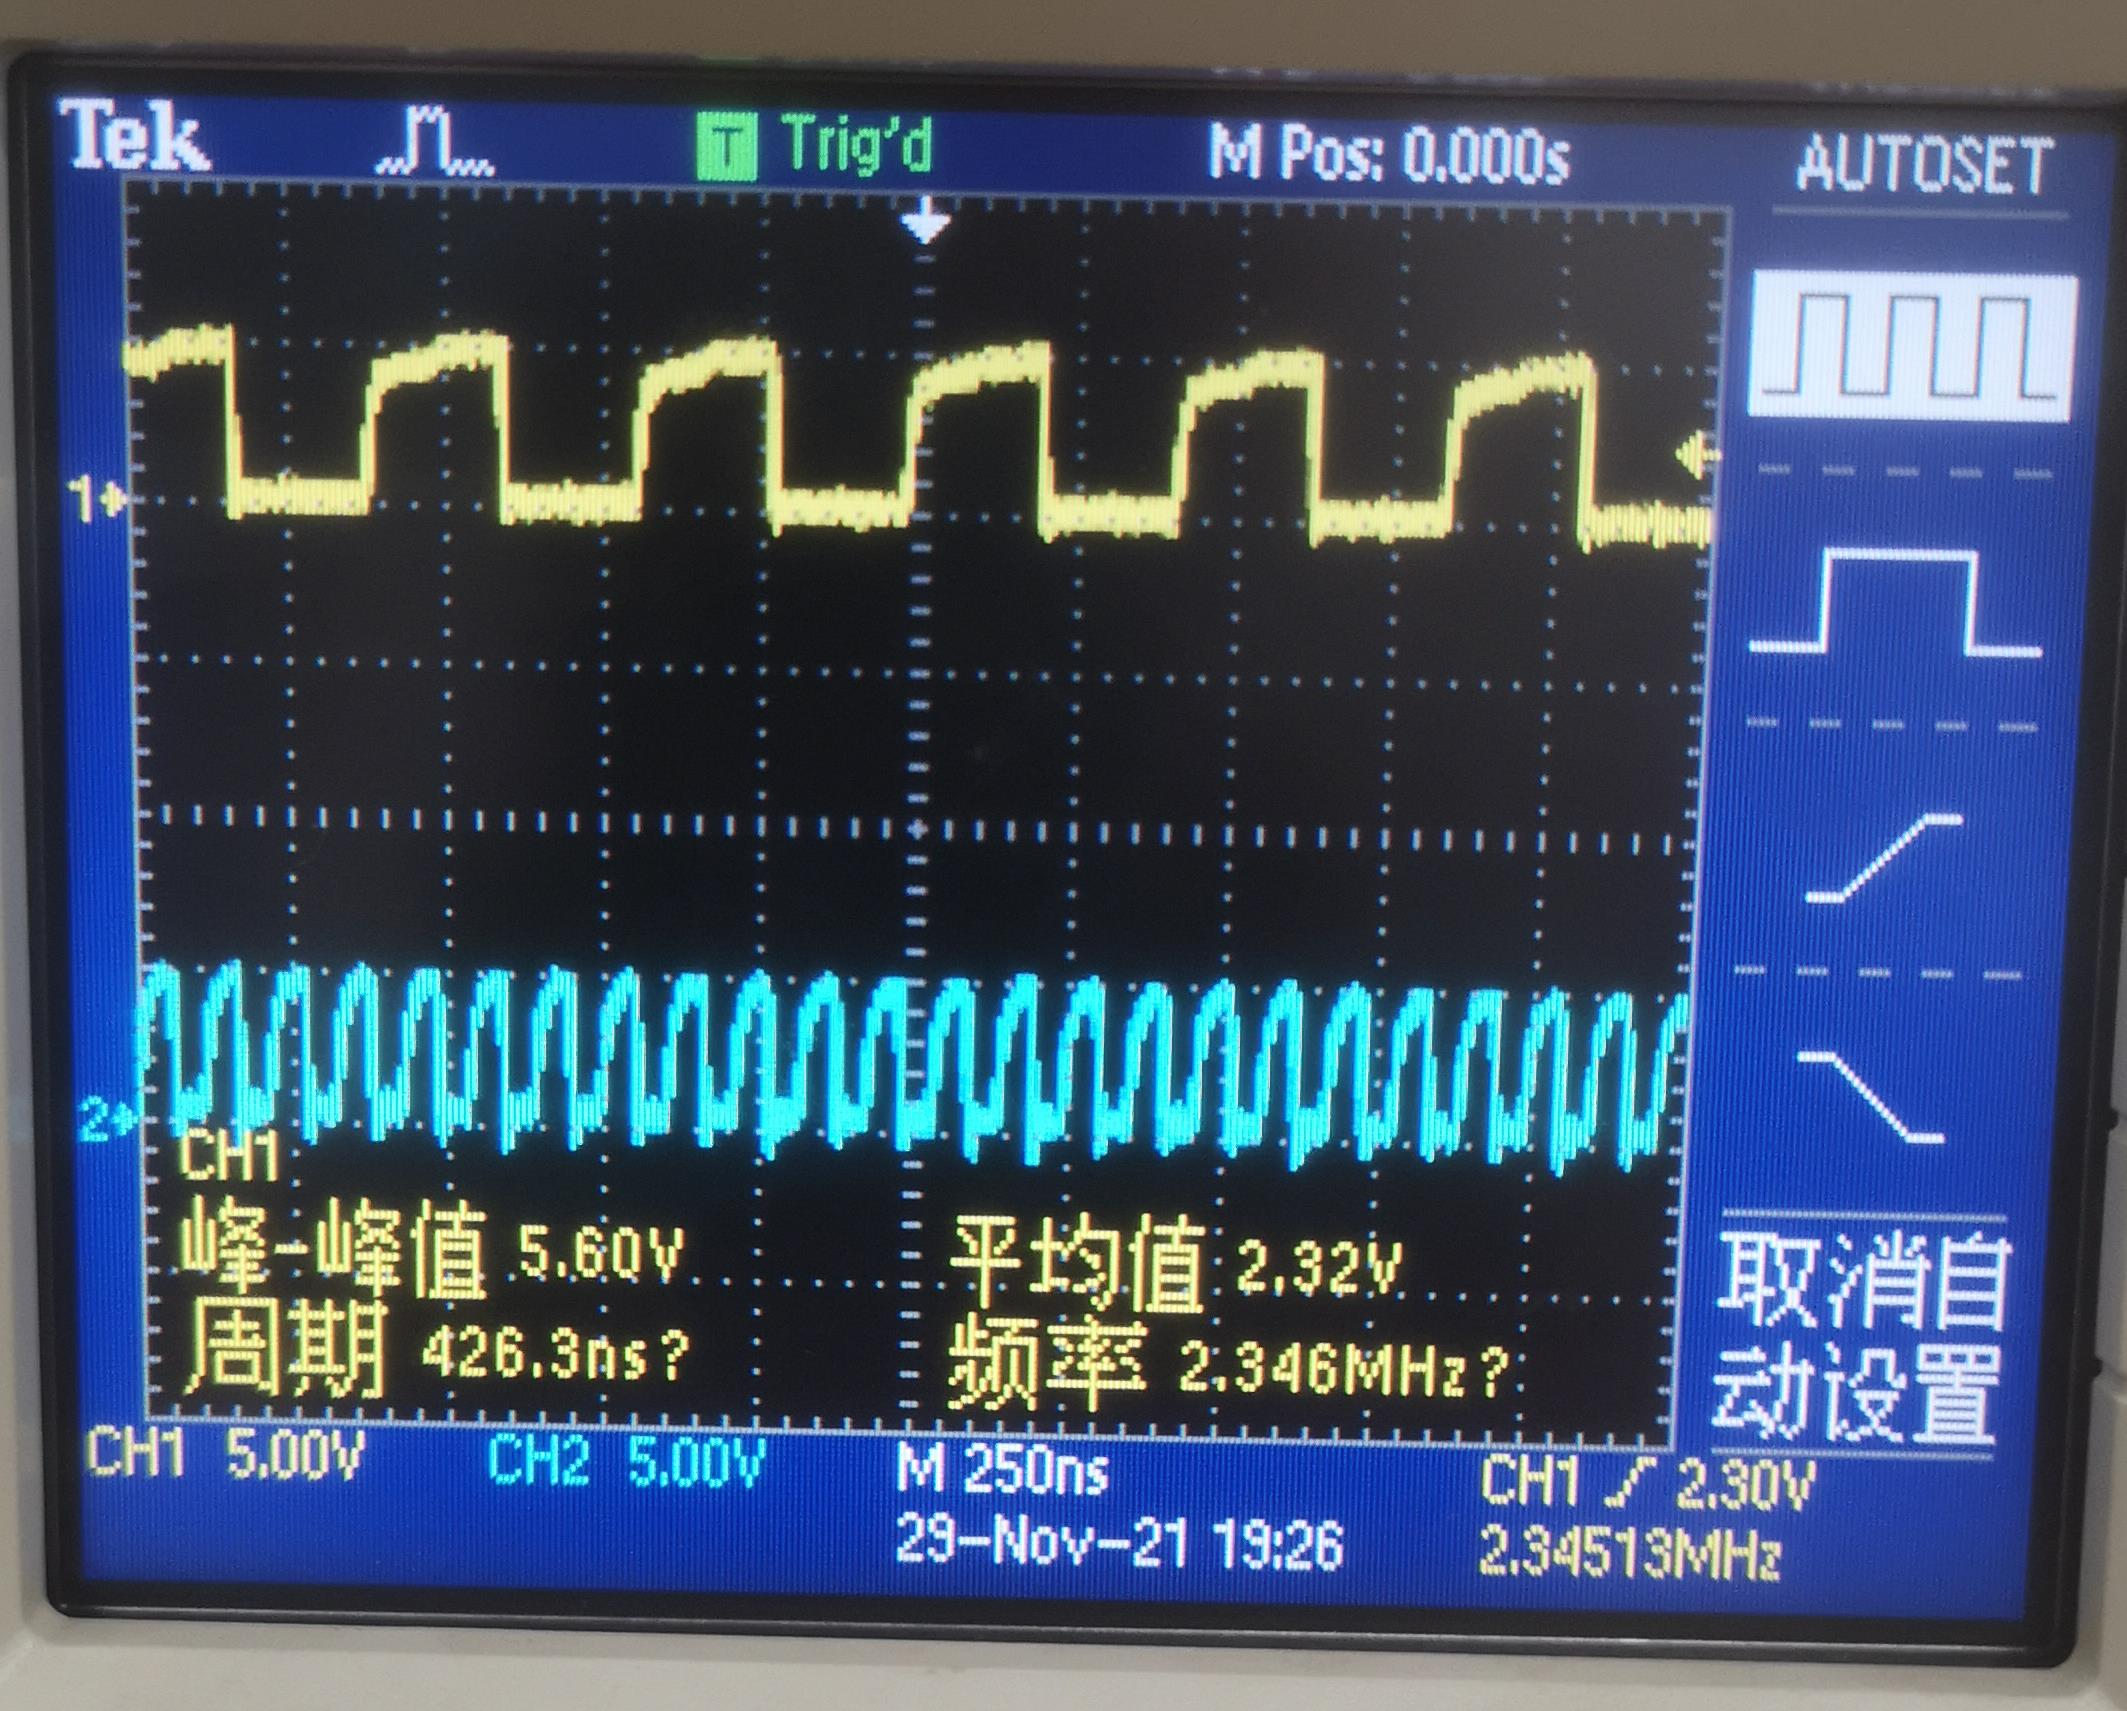
\includegraphics[width=.4\linewidth]{pic/3.jpg}
    		\caption{$Q_{B}$和$Q_{D}$波形图
    		}
    	\end{figure}
    	\begin{figure}[H]
    		\centering
    		\hspace{2em}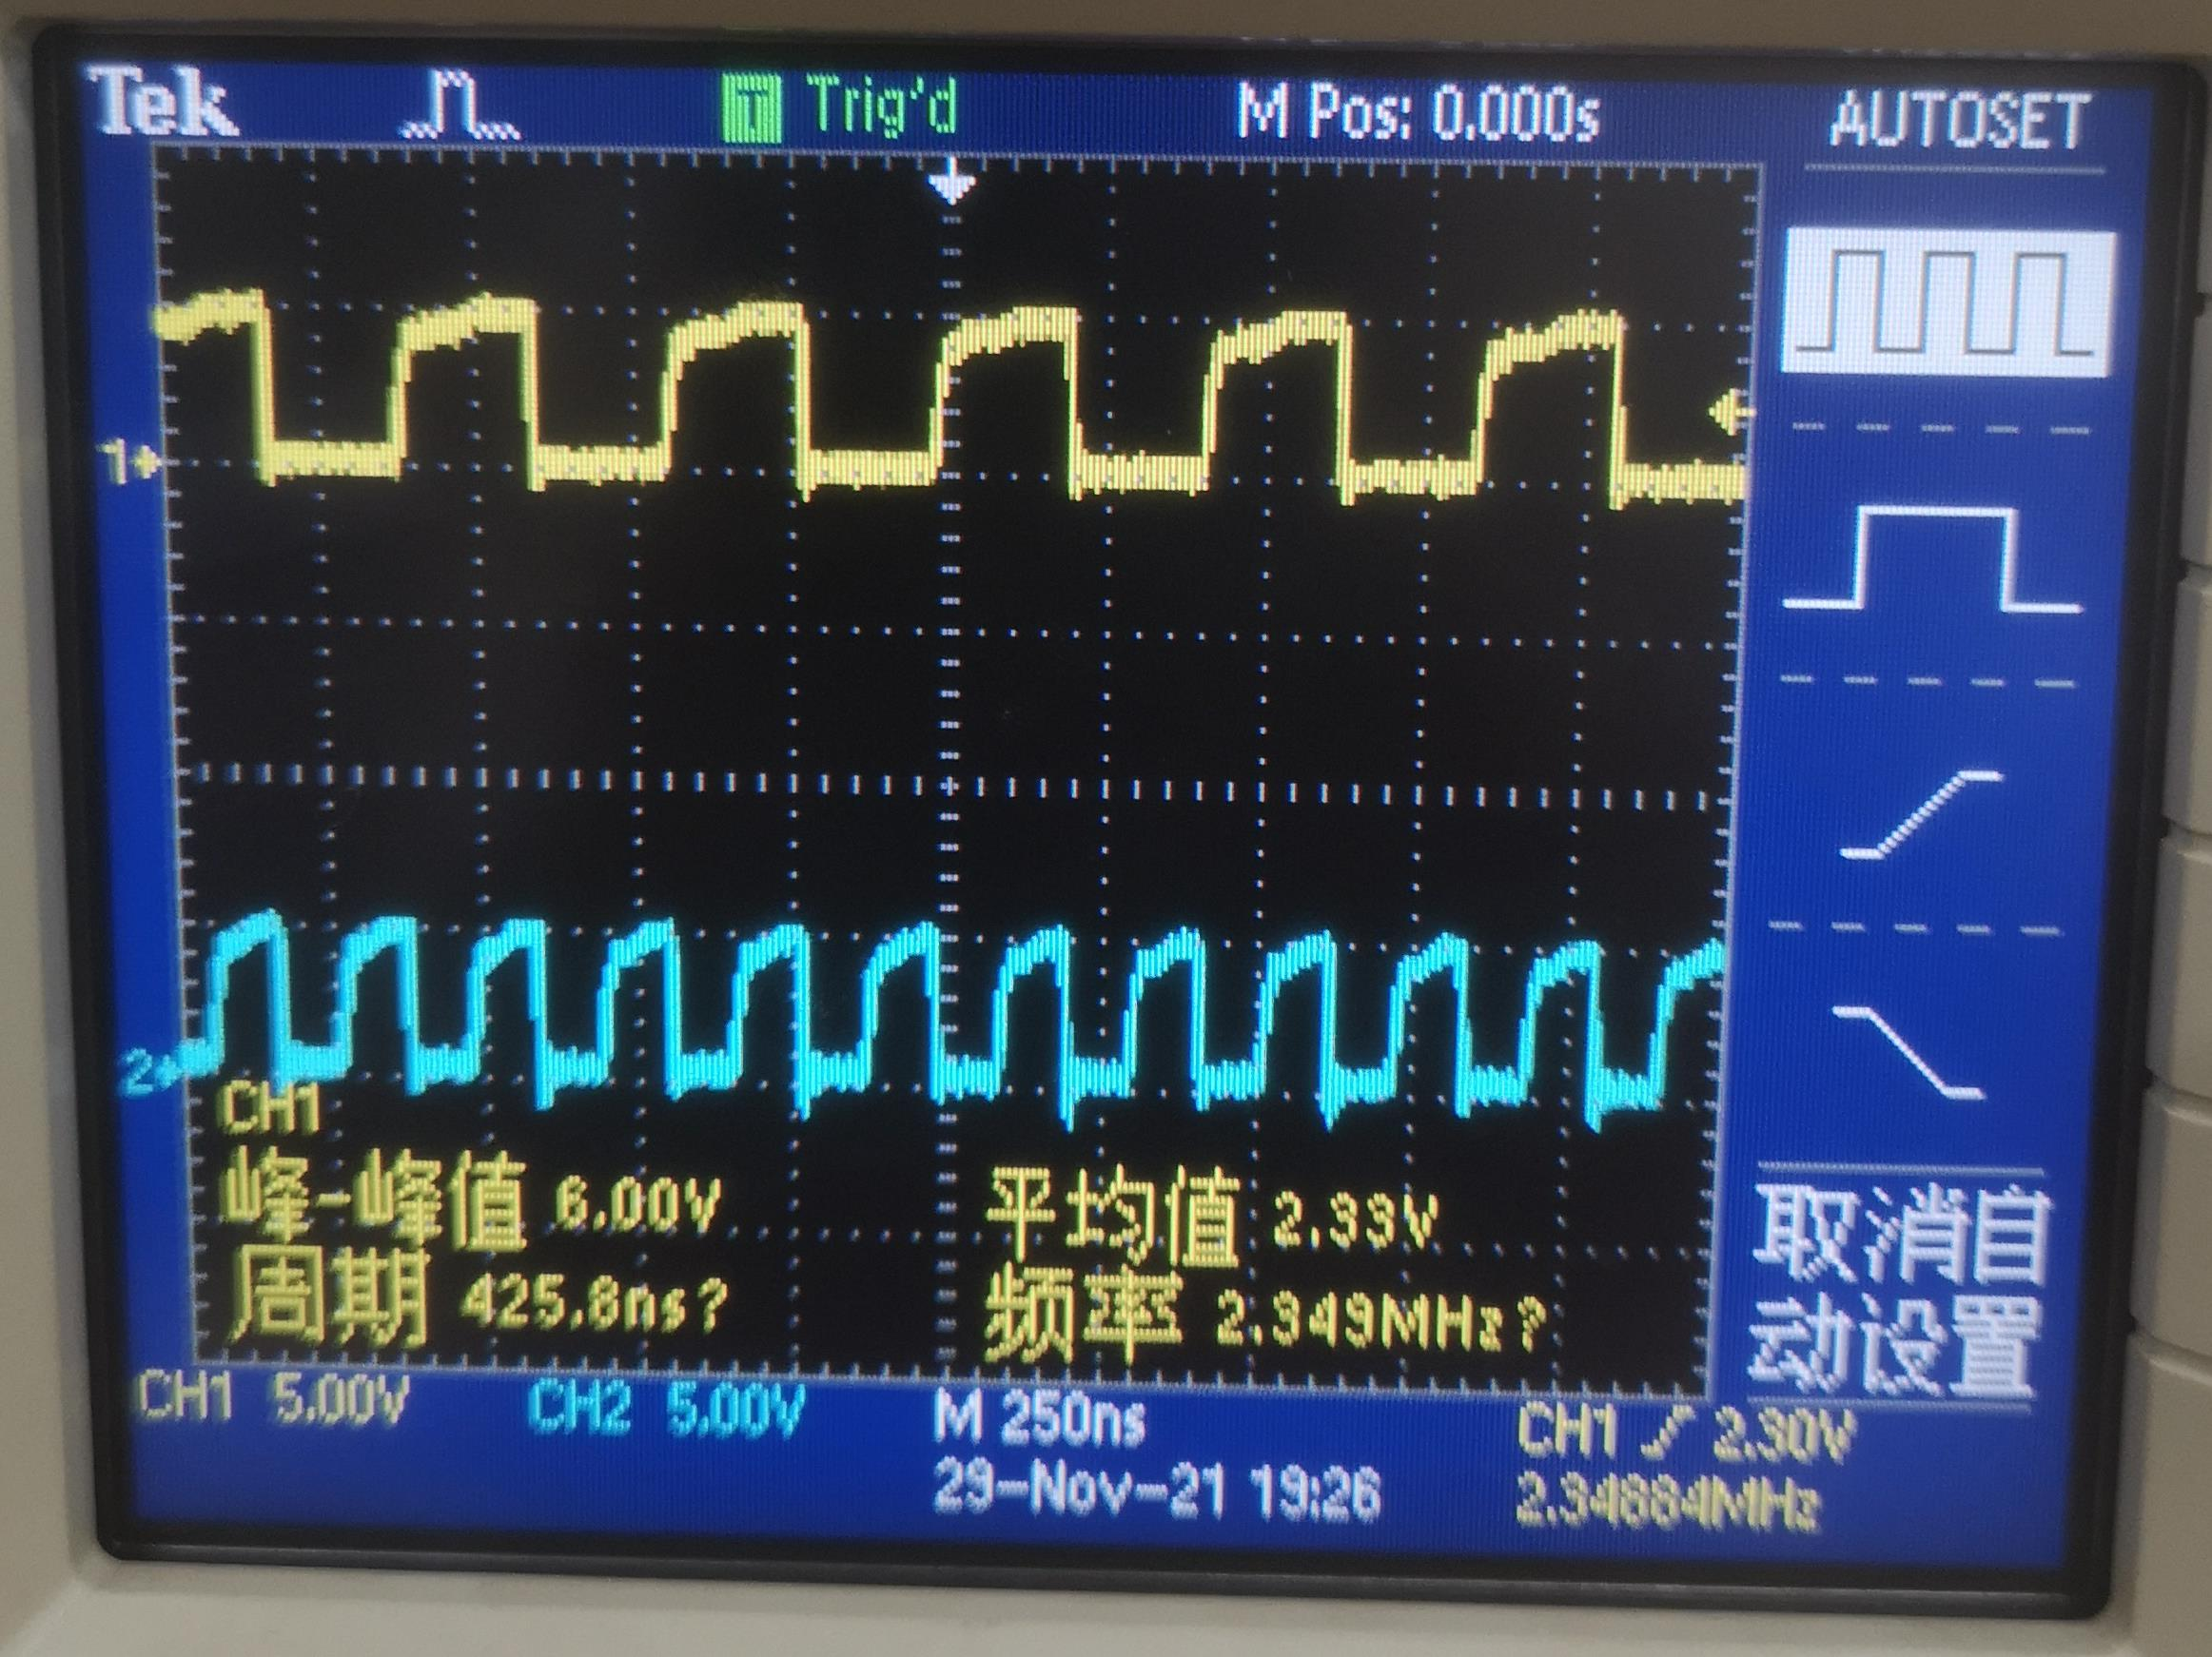
\includegraphics[width=.4\linewidth]{pic/4.jpg}
    		\caption{$Q_{B}$和$Q_{D}$波形图
    		}
    	\end{figure} 
    \par 由$Q_{A}$和$Q_{D}$的波形图我们可得$\tau_{A}=52.0ns,\tau_{D}=427.6ns$
    \par 因此我们由$Q_{A}$可得$t_{pd}=\dfrac{\tau_{A}}{12}\approx4.33ns$,由$Q_{D}$可得$t_{pd}=\dfrac{\tau_{D}}{96}\approx4.45ns$   
	\section{思考题}
	\noindent
	\textbf{1.测量与非门的空载功耗有何实际意义?为什么门电路的功耗与输入信号频率有关?
}
	\par 答:TTL集成门电路工作时,器件本身要消耗一定的功率,功耗也是门电路的特性指标之一。由于功耗随负载的不同而变化,为了简便起见,通常以空载功耗来表征。空载功耗是与非门空载时的电源总电流与电源电压的乘积。当输出为低电平时的空载功耗称为导通功耗,用$P_{ON}$表示;当输出为高电平时的空载功耗称为截止功耗,用$P_{OFF}$表示。与非门的平均功耗与门电路的工作频率有关,工作频率越高,平均功耗就越大。这是由于与非门由低电平快速转变为高电平时,$T_3$退出饱和状态之前$T_4$就导通了,会在很短的瞬间使电源和地之间出现一个低阻回路,形成一个尖峰电流,这个电流将增加与非门的平均功耗。\\
    \textbf{2.与非门的噪声容限与哪些参量有关?}
    \par 答:高电平噪声容限=最小输出高电平电压-最小输入高电平电压,低电平噪声容限=最大输入低电平电压-最大输出低电平电压,与非门的噪声容限=min{高电平噪声容限,低电平噪声容限}。与非门的噪声容限与环境温度,电路级联状态,电源电压,数字电路的反应速度,传输延迟时间,施加干扰波形,以及器件的阈值电压等因素有关。\\
    \textbf{3.本实验的环形振荡器是由三级与非门组成的直耦反馈环路,如果由一级或偶数级与非门组成直耦反馈环路,能否产生振荡?为什么?}
    \par 答:如果只有一级,可以产生振荡,但因为$T=2t_{pd}$,而$t_{pd}$很小,所以会导致振荡频率非常高;但是偶数级不能形成振荡,因为这样会形成一个稳定的状态而不会振荡。
\end{document} 
